\documentclass[11pt]{article}
\usepackage{graphicx,natbib,amsmath}

\setlength{\textheight}{24.5cm}
\setlength{\textwidth}{16.5cm}
\setlength{\topmargin}{-14mm}
\setlength{\evensidemargin}{-2mm}
\setlength{\oddsidemargin}{-2mm}
\setlength{\headsep}{4mm}

\def\nH{n_{\langle\rm H\rangle}}
\def\nHi{n_{\langle\rm H\rangle,i}}
\def\nHleft{n_{\langle\rm H\rangle,1}}
\def\nHright{n_{\langle\rm H\rangle,I}}
\def\nHim1{n_{\langle\rm H\rangle,i-1}}
\def\nHip1{n_{\langle\rm H\rangle,i+1}}
\def\Vl{V_{\ell}}
\def\Nl{N_{\ell}}
\def\rhod{\rho_{\rm d}}
\def\ek{\epsilon_k}
\def\pdiff#1#2{\frac{\partial #1}{\partial #2}}
\def\rhogr{\rho_{\rm gr}}
\def\Dd{D_{\!d}}
\def\apj{ApJ}
\def\pasp{PASP}
\def\pasj{PASJ}
\def\araa{ARA\&A}
\def\aap{A\&A}
\def\aaps{A\&AS}
\def\apjl{ApJL}
\def\apjs{ApJS}
\def\mnras{MNRAS}
\def\aj{AJ}
\def\nat{Nature}
\def\icarus{Icarus}
\def\pasa{PASA}
\DeclareRobustCommand{\Eins}{\text{\usefont{U}{bbold}{m}{n}1}}

\def\la{\mathrel{\mathchoice {\vcenter{\offinterlineskip\halign{\hfil
$\displaystyle##$\hfil\cr<\cr\sim\cr}}}
{\vcenter{\offinterlineskip\halign{\hfil$\textstyle##$\hfil\cr
<\cr\sim\cr}}}
{\vcenter{\offinterlineskip\halign{\hfil$\scriptstyle##$\hfil\cr
<\cr\sim\cr}}}
{\vcenter{\offinterlineskip\halign{\hfil$\scriptscriptstyle##$\hfil\cr
<\cr\sim\cr}}}}}
\def\ga{\mathrel{\mathchoice {\vcenter{\offinterlineskip\halign{\hfil
$\displaystyle##$\hfil\cr>\cr\sim\cr}}}
{\vcenter{\offinterlineskip\halign{\hfil$\textstyle##$\hfil\cr
>\cr\sim\cr}}}
{\vcenter{\offinterlineskip\halign{\hfil$\scriptstyle##$\hfil\cr
>\cr\sim\cr}}}
{\vcenter{\offinterlineskip\halign{\hfil$\scriptscriptstyle##$\hfil\cr
>\cr\sim\cr}}}}}


\begin{document}

\begin{center}
\resizebox{!}{9mm}{\huge\sf DIFFUSE}\\[4mm]
\resizebox{!}{4.5mm}{\huge An implicit/explicit/time-independent 
                            second-order diffusion solver}\\[3mm]
\resizebox{!}{5mm}{\huge\sf Peter Woitke}\\[3mm]
\resizebox{!}{3.5mm}{\huge November 2017}\\*[8mm]

\paragraph{Definitions}{\ }\\[2mm]

\begin{tabular}{l|l|c}
\hline
symbol  & description & unit\\
\hline
$z$                       & vertical coordinate    & cm\\
$\nH$                     & hydrogen nuclei density & cm$^{-3}$\\
$\rho = \mu_{\rm H}\,\nH$  & gas mass density       & g\,cm$^{-3}$\\
$\mu_{\rm H}=\sum_k m_k\ek$  & proportionality constant & g\\ 
$m_k$                     & mass of element $k$     & g\\
%$T$                       & gas temperature        & K\\
%$p = \frac{\rho}{\mu}kT$  & gas pressure           & dyn\,cm$^{-2}$\\
%$\mu$                     & mean gas particle mass & g\\
$\ek$                     & abundance of element $k$ & -\\[-1mm]
                          & with respect to hydrogen &\\
$D$                       & diffusion coefficient  & cm$^2$\,s$^{-1}$\\
\hline  
\end{tabular}

\end{center}

\bigskip
\section{The diffusion problem}

The motion of elements in a planetary atmosphere will be considered
to be diffusive. There are two effects to consider: (a) gains and
losses through the boundaries and (b) local source and sink terms due
to the formation, drift, and evaporation of solids or liquids
particles (precipitation). 

Examples for processes of type (a) are the outgasing of elements from
the rock forming the surface of the planet (the lower boundary of the
atmosphere), and the loss of certain elements at the top of the
atmosphere (Jeans escape).

The diffusive flux $\vec{j}_k\rm\ [cm^{-2} s^{-1}]$ of an element $k$ is
given by its concentration gradient, which is known as Fick's first law 
\citep[see e.g.][]{Bringuier2013} 
\begin{equation}
  \vec{j}_k = -\nH D\,\nabla\ek
\end{equation}
and the local gains and losses  $\rm [cm^{-3} s^{-1}]$ on the right
hand side of the continuity equation for element $k$ is given by the
divergence of the diffusive flux (Fick's second law) as
\begin{equation}
  \pdiff{(\nH\,\ek)}{t} + \nabla(\vec{v}\,\nH\ek) 
   ~=~ -\nabla\vec{j}_k + S_k \ ,
\end{equation}
where $S_k$ are additional local source/sink terms
$\rm[cm^{-3}\,s^{-1}]$, for example when dust grains grow or evaporate
in the atmosphere. Combining these two equations we find the
diffusion-reaction equation
\begin{equation}
  \pdiff{(\nH\,\ek)}{t} + \nabla(\vec{v}\,\nH\ek) 
   ~=~ \nabla\left(\nH D\,\nabla\ek\right) + S_k \ .
\end{equation}

\subsection{Static planeparallel atmosphere}

We assume that the gas in the atmosphere is quasi-static $\vec{v}=0$, and
we assume the atmosphere to have plane-parallel geometry
$\nabla\to\frac{d}{dz}$, in which case we find
\begin{equation}
  \boxed{\frac{d(\nH\,\ek)}{dt} ~=~ 
     \frac{d}{dz}\left(\nH D\,\frac{d\ek}{dz}\right)  + S_k}
  \label{basic}
\end{equation}

\subsection{The diffusion constant}

The gas-kinetic diffusion constant is given by
\begin{equation}
  D_{\rm micro} ~=~ \frac{1}{3}\,v_{\rm th}\,\ell \ ,
\end{equation}
where $\ell=1/(\sigma\,n)$ is the mean free path, $n$ the total
gas particle density and $\sigma\approx 2.1\times 10^{-15}\rm\,cm^2$
a typical cross-section for a H$_2$-rich gas where the thermal
velocity is defined as $v_{\rm th}=\sqrt{8 k T/(\pi\mu)}$
\citep{Woitke2003}.  This microphysical diffusion constant is often 
negligible in planetary atmospheres. 

Instead, mixing by turbulent motions is usually the dominant mixing
process. We describe this mixing by an effective diffusion
coefficient which normally is much larger than $D_{\rm micro}$. The
turbulent diffusion coefficient is roughly given by
\begin{equation}
  D_{\rm mix} ~\approx~ \langle v_z\rangle\,H_p \ ,
\end{equation} 
where $\langle v_z\rangle$ is the root-mean-square average of vertical
velocities in the atmosphere, at height $z$. In the convective layer,
$\langle v_z\rangle\approx v_{\rm conv}$ is the convective velocity
which is a part of the stellar atmosphere model and results from the
application of mixing length theory.  Above the convective layer,
where the Schwarzschild criterion for convection is false, $\langle
v_z\rangle$ will decrease rapidly with increasing $z$, but will not be
entirely zero due to convective overshoot. We apply a powerlaw in
$\log p$ to approximate this behaviour
\begin{equation}
  \log \langle v_z\rangle ~=~ \log v_{\rm conv} 
                          - \beta\cdot\max\{0,\log p_{\rm conv}-\log p(z)\}
\end{equation}
with free parameter $\beta\approx 0.5\,...\,2.2$ \citep{Ludwig2002,Lee2015}.
At high altitudes, $n$ becomes small and hence $D_{\rm micro}$ large,
and $\langle v_z\rangle$ becomes small, hence $D_{\rm mix}$ small.
We take both processes into account by summing up 
\begin{equation}
  D ~=~ D_{\rm mix} + D_{\rm micro} \ .
\end{equation}

\section{Solution method}

\subsection{Vertical grid and discretisation of derivatives}
We introduce an ascending vertical grid $z_i\ (i=1, ...\,,I)$. The first and
second derivatives of any quantity $f(z_i)=f_i$ at grid point $z_i$ 
are approximated as
\begin{eqnarray}
  \frac{df_i}{dz}     
  &=& d^{\,l,1}_if_{i-1} + d^{\,m,1}_if_i + d^{\,r,1}_if_{i+1} \\ 
  \frac{d^2f_i}{dz^2} 
  &=& d^{\,l,2}_if_{i-1} + d^{\,m,2}_if_i + d^{\,r,2}_if_{i+1} \ ,
\end{eqnarray}
i.e.\ as linear combinations of the function values on the
neighboring grid points, where e.g.\ $d^{\,l,1}_i$ is the coefficient
for the first derivative on the point left of the grid point $i$,
$d^{\,m,1}_i$ the same on the mid point and $d^{\,r,1}_i$ the same on
the point right of grid point $i$. Similar, for the second derivative,
the coefficients are $d^{\,l,2}_i$, $d^{\,m,2}_i$ and
$d^{\,r,2}_i$. Using a second-order polynomial approximation for
function $f(z)$ the coefficients are given by
\begin{eqnarray}
  d^{\,l,1}_i &=& -\,\frac{h^r_i}{(h^r_i+h^l_i)\,h^l_i}   \\
  d^{\,m,1}_i &=& +\,\frac{h^r_i-h^l_i}{h^l_i h^r_i}     \\
  d^{\,r,1}_i &=& +\,\frac{h^l_i}{(h^r(i)+h^l_i)\,h^r_i}  \\
  d^{\,l,2}_i &=& +\,\frac{2}{(h^r_i+h^l_i)\,h^l_i}      \\
  d^{\,m,2}_i &=& -\,\frac{2}{h^r_i h^l_i}             \\
  d^{\,r,2}_i &=& +\,\frac{2}{(h^r_i+h^l_i)\,h^r_i}      
\end{eqnarray}   
where $h^l_i=z_i-z_{i-1}$ and $h^r_i=z_{i+1}-z_i$ are the l.h.s.\
and the r.h.s.\  grid point distances. Note that for the special case of
an equidistant grid, we have $h=h^l_i=h^r_i$ and hence
\begin{eqnarray}
  \frac{df_i}{dz}     &=& \frac{f_{i+1}-f_{i-1}}{2h} \\
  \frac{d^{\,2}\!f_i}{dz^2} &=& \frac{f_{i+1}-2f_i+f_{i-1}}{h^2}
\end{eqnarray}
The above equations are valid for grid points $i=2,\,...\,,I-1$.
For the first derivative at the boundaries we write
\begin{eqnarray}
  \frac{df_1}{dz}     
  &=& d^{\,l,1}_1f_{1} + d^{\,m,1}_1f_{2} + d^{\,r,1}_1f_{3} \\ 
  \frac{df_1}{dz}     
  &=& d^{\,l,1}_If_{I-2} + d^{\,m,1}_If_{I-1} + d^{\,r,1}_If_{I} 
\end{eqnarray}
which is also second-order accuracy by using the information on the 
3 leftmost or 3 rightmost grid points, respectively.
The coefficients are given by
\begin{eqnarray}
      d^{\,l,1}_1 &=& -\frac{h_2+h_3}{h_2 h_3} \\
      d^{\,m,1}_1 &=&  \frac{h_3}{h_2(h_3-h_2)} \\
      d^{\,r,1}_1 &=& -\frac{h_2}{h_3(h_3-h_2)} \\
      d^{\,r,1}_I &=&  \frac{h_{I-1}+h_{I-2}}{h_{I-1} h_{I-2}} \\
      d^{\,m,1}_I &=& -\frac{h_{I-2}}{h_{I-1}(h_{I-2}-h_{I-1})} \\
      d^{\,l,1}_I &=&  \frac{h_{I-1}}{h_{I-2}(h_{I-2}-h_{I-1})}
\end{eqnarray}
where $h_2=z_2-z_1$, $h_3=z_3-z_1$, $h_{I-1}=z_I-z_{I-1}$ and 
$h_{I-2}=z_I-z_{I-2}$.

\subsection{Spatial derivatives}

The diffusion term at grid point $z_i\;(i=2,\,...\,,I-1)$ 
is numerically resolved as
\begin{eqnarray}
  \frac{d}{dz}\left(\nHi D_i\frac{d\epsilon_{k,i}}{dz}\right) 
  &=&  \frac{d(\nHi D_i)}{dz}\,\frac{d\epsilon_{k,i}}{dz}
       ~+~\nHi D_i\frac{d^2\epsilon_{k,i}}{dz^2} \nonumber\\
  &=& \left(d^{\,l,1}_i\nHim1 D_{i-1} 
          + d^{\,m,1}_i\nHi   D_i 
          + d^{\,r,1}_i\nHip1 D_{i+1}\right)\nonumber\\
  &&
   \!\!\!\cdot \left(d^{\,l,1}_i\epsilon_{k,i-1} 
                   + d^{\,m,1}_i\epsilon_{k,i} 
                   + d^{\,r,1}_i\epsilon_{k,i+1} \right) \nonumber\\
  &+& \nHi D_i \left(d^{\,l,2}_i\epsilon_{k,i-1} 
                   + d^{\,m,2}_i\epsilon_{k,i} 
                   + d^{\,r,2}_i\epsilon_{k,i+1} \right) \label{Acoeff}
\end{eqnarray}
and the diffusive fluxes accross the lower and upper boundaries are
\begin{eqnarray}
 j_{k,1} &=& -\nHleft D_1 \frac{d\epsilon_{k,1}}{dz}
        ~=~ -D_1\nHleft \left(d^{\,l,1}_1\epsilon_{k,1} 
                            + d^{\,m,1}_1\epsilon_{k,2} 
                            + d^{\,r,1}_1\epsilon_{k,3}\right)\\
 j_{k,I} &=& -\nHright D_I \frac{d\epsilon_{k,I}}{dz}
        ~=~ -D_I\nHright \left(d^{\,l,1}_I\epsilon_{k,I-2} 
                            + d^{\,m,1}_I\epsilon_{k,I-1} 
                            + d^{\,r,1}_I\epsilon_{k,I}\right) \ .
\end{eqnarray}

\subsection{Boundary conditions}

As boundary conditions, we have three options. For example,
considering the lower boundary: 
\begin{enumerate}
\item fixed concentration: \hspace*{10.5mm}$\epsilon_{k,1}$ is a given constant
\item fixed flux: \hspace*{27mm}$j_{k,1}$ is a given constant
\item fixed outflow rate: ~~The flux through a boundary is assumed to be
  proportional to the concentration of species $k$ at the boundary,
  e.g.
  \begin{equation}
    j_{k,1} = \beta_k\,\nHleft\,\epsilon_{k,1}\,v_{k,\rm th}  
    \quad\quad{\rm[cm^{-2}s^{-1}]}
  \end{equation}      
  where the $\beta_k$ is a given probability (fixed value) and 
  $v_{k,\rm th}$ is the speed at which the particles of kind $k$
  move through the boundary (also fixed value).
\end{enumerate} 

\subsection{Explicit time-integration}
A straightforward way to integrate Eq.~(\ref{basic}),
using a timestep $\Delta t$, is the following explicit scheme
\begin{eqnarray}
  f_i^{n} &=& f_i^{n-1} + \Delta t \frac{df_i^{n-1}}{dt}  
\end{eqnarray}
where $f^n_i$ is some quantity on grid point $i$ at time $t^n$
and $f^{n-1}_i$ is the quantity on grid point $i$ at time $t^{n-1}$
with $t^n=t^{n-1}+\Delta t$. In consideration of Eq.~(\ref{basic}),
this leads to
\begin{eqnarray}
  \epsilon_{k,i}^{n} &=& \epsilon_{k,i}^{n-1} + \Delta t 
     \left(\sum\limits_{j=1}^{I} A_{ij}\epsilon_{k,j}^{n-1}
           + \frac{S_i^{n-1}}{\nHi}\right)  \ ,
  \label{explicit}
\end{eqnarray}
where $\mathbf{A}$ is a tri-diagonal matrix, the elements $A_{ij}$
of which are given by Eq.~(\ref{Acoeff}). Equation~(\ref{explicit})
applies to the grid points $i=2,\,...\,,I-1$, but not to the boundaries. 
On the boundary points, the following equations are applied
depending on the choice of boundary conditions, here for example the
lower boundary

\newpage
\begin{enumerate}
\item fixed concentration:
      ~~$\displaystyle\epsilon_{k,1}^{n} = \epsilon_{k,1}^{n-1}$
\item fixed flux:\hspace*{19.5mm}
      $\displaystyle\epsilon_{k,1}^{n} = \frac{1}{d^{\,l,1}_1}
       \left(-\frac{j_{k,1}}{D_1\nHleft} 
             -d^{\,m,1}_1\epsilon^n_{k,2} 
             -d^{\,r,1}_1\epsilon^n_{k,3}\right)$
\item fixed outflow rate: From
      ~~$j_{k,1} = \displaystyle -D_1\nHleft\left(
              d^{\,l,1}_1\epsilon_{k,1}^{n} 
             +d^{\,m,1}_1\epsilon^n_{k,2} 
             +d^{\,r,1}_1\epsilon^n_{k,3}\right)
      = \beta_k\,\nHleft\,\epsilon_{k,1}\,v_{k,\rm th}$\\
      we find\\
    \hspace*{37mm}$\displaystyle\epsilon_{k,1}^{n} = 
       \frac{-d^{\,m,1}_1\epsilon^n_{k,2} 
             -d^{\,r,1}_1\epsilon^n_{k,3}}
            {\displaystyle d^{\,l,1}_1+\frac{\beta_k\,v_{k,\rm th}}{D_1}}$
  \ .
\end{enumerate} 
To guanantee numerical stability, the explicit timestep must be 
limited by $\alpha\leq0.5$ according to
\begin{equation}
  \Delta t ~=~ \alpha\;\min_{i\,=\,2,\,...\,,I}~ 
               \frac{(z_i-z_{i-1})^2}{\frac{1}{2}(D_i+D_{i-1})} \ .
  \label{tstep}
\end{equation}

\subsection{Implicit integration}
To avoid the timestep limitation, and to guarantee numerical stability
for much larger timesteps, an implicit integration scheme will be used
\begin{eqnarray}
  f_i^{n} &=& f_i^{n-1} + \Delta t \frac{df_i^{n}}{dt}  
\end{eqnarray}
which is a system of linear equations for the unknowns $f_i^{n}$.
In consideration of Eq.~(\ref{basic}), we have
\begin{eqnarray}
  \epsilon_{k,i}^{n} &=& \epsilon_{k,i}^{n-1} + \Delta t 
     \left(\sum\limits_{j=1}^{I} A_{ij}\epsilon_{k,j}^{n}
           + \frac{S_i^{n-1}}{\nHi}\right) 
\end{eqnarray}
We re-write this equation more generally, including the
boundary conditions as, by means of another unit-free matrix as 
\begin{eqnarray}
  \mathbf{B}\,\vec{\epsilon}_k^{\;n} &=& \vec{R}_{k} \ ,
  \label{implicit}
\end{eqnarray}
where we have
\begin{equation}
  B_{ij} = \left(\Eins-\Delta t \mathbf{A}\right)_{ij} 
  \quad\mbox{and}\quad R_{k,i} = \epsilon_{k,i}^{n-1} 
  + \Delta t\frac{S_i^{n-1}}{\nHi}
  \quad\quad\mbox{for $i=2,\,...\,,I-1$}
\end{equation}
and, depending on boundary conditions, for example at the lower boundary
\begin{enumerate}
\item fixed concentration: 
      ~$B_{11}=1$ 
      and $R_{k,1}=\epsilon_{k,1}^{n-1}$
\item fixed flux:
      \hspace*{18.5mm}$B_{11}=1$, 
      $B_{12}={d^{\,m,1}_1}/{d^{\,l,1}_1}$,
      $B_{13}={d^{\,m,1}_1}/{d^{\,l,1}_1}$, 
      and $R_{k,1}=-j_{k,1}/\big(\nHleft D_1 d^{\,l,1}_1\big)$
\item fixed outflow rate:
      \hspace*{4mm}$B_{11}=1+\beta_k\,v_{k,\rm th}/\big(D_1 d^{\,l,1}_1\big)$, 
      $B_{12}={d^{\,m,1}_1}/{d^{\,l,1}_1}$,
      $B_{13}={d^{\,m,1}_1}/{d^{\,l,1}_1}$\\
      \hspace*{37mm}and $R_{k,1}=0$  \ .
\end{enumerate}
We can now perform an implicit timestep according to Eq.~(\ref{implicit}) 
as
\begin{eqnarray}
  \vec{\epsilon}_k^{\;n} &=& \mathbf{B}^{-1}\,\vec{R}_{k}
  \label{implicit2}
\end{eqnarray}
where $\mathbf{B}^{-1}$ is the inverse of the matrix $\mathbf{B}$.  As
long as the the spatial grid points $z_i$, the densities $\nHi$ and
diffusion constants $D_i$, the constants involved in the boundary
conditions (e.g. $j_{k,1}$ or $\beta_k$), and the timestep $\Delta t$
does not change, we need to perform the matrix inversion only
once. Successive time steps are then performed by simply incrementing
$n$, re-computing the vector $\vec{R}_{k}$, and applying again 
Eq.~(\ref{implicit2}). $\mathbf{B}^{-1}$ is also usually the same
for all elements $k$ to be diffused.

This favourable property of $\mathbf{B}$ makes the computation
of implicit timesteps actually very fast. We note, however, that
$\mathbf{B}^{-1}$, in general, is a full $I\times I$ matrix where all
entries are positive $(\mathbf{B}^{-1})_{ij}>0$. This leads to a very
stable numerical behaviour for arbitrary time steps. In contrast, the
matrix $\mathbf{A}$ has positive entries along the main diagonal, but
negative entries along both semi-diagonals, which leads to numerical
instabilities when the time step is too large.

\section{Test results}

Figures \ref{fig1} to \ref{fig4} show a few test problems on domain
$z=0\,...\,1$, with constant $\nH=1$ and $D=1$. The third and forth
test problem have overplotted analytic solutions. All tests use
an equidistant $z$-grid with 101 points, use the implicit solver, 
and can be computed within less than 1\, CPU-sec.

\begin{figure}[!p]
\centering
\vspace*{-5mm}
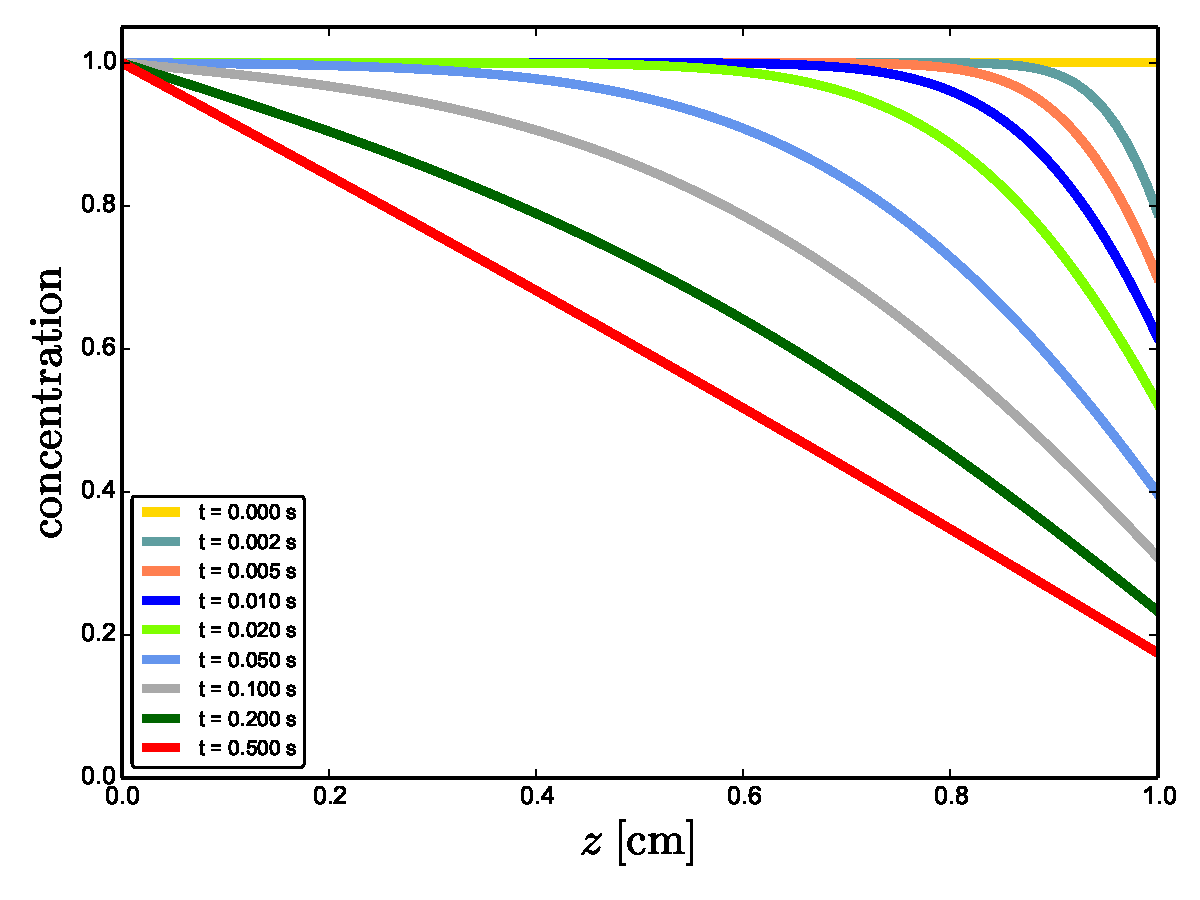
\includegraphics[width=14cm]{test1.pdf}\\[-5mm]
\caption{Test problem with fixed concentration on the left
  $(\epsilon=1)$, and fixed outflow rate $(\beta=5)$ on the
  right. Near t=0.5\,s, the concentration has reached a steady state
  where elements are constantly transported rightways.}
\label{fig1}
\end{figure}

\begin{figure}
\centering
\vspace*{-5mm}
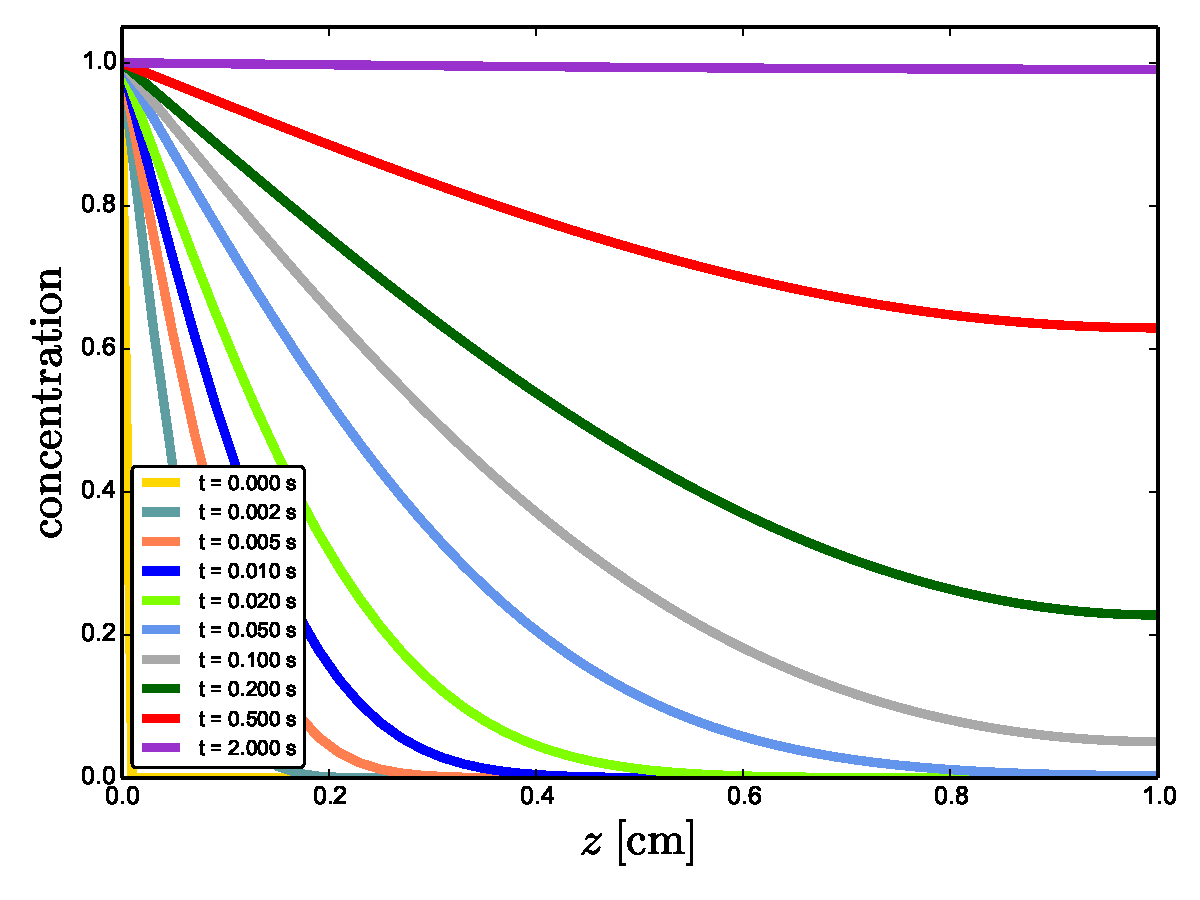
\includegraphics[width=14cm]{test2.pdf}\\[-5mm]
\caption{Test problem with fixed concentration on the left
  $(\epsilon=1)$, and fixed flux $(j=0)$ on the right.  The
  time-independent solution $\epsilon=1$ is reached at about 2\,s.}
\label{fig2}
\end{figure}

\begin{figure}
\centering
\vspace*{-5mm}
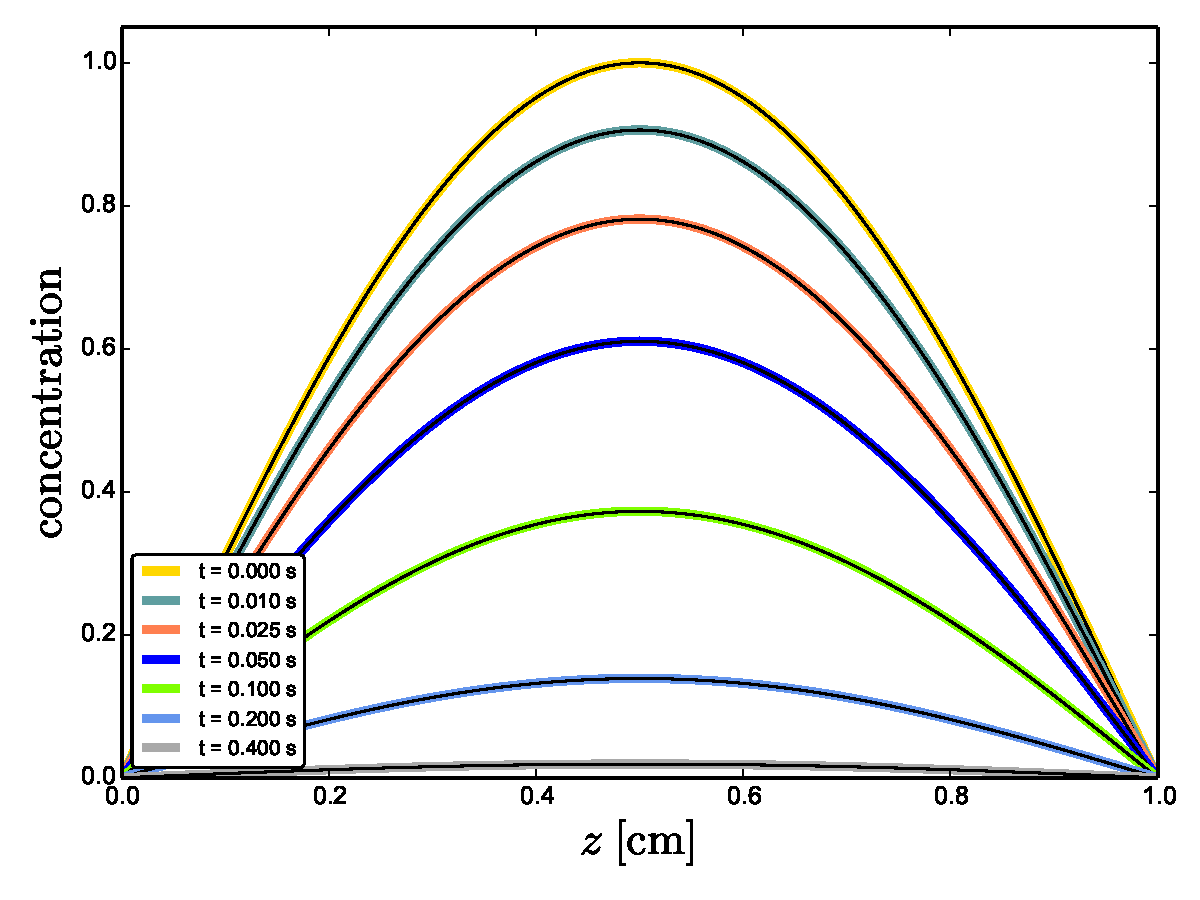
\includegraphics[width=14cm]{test3.pdf}\\[-5mm]
\caption{Test problem with fixed concentrations on the left and right
  sides $(\epsilon=0)$. The thin black lines overplot the analytic
  solution $\epsilon(z,t)=\exp(-\omega t) \sin(k z)$ with $k=\pi$ and
  $\omega=D k^2$.}
\label{fig3}
\end{figure}

\begin{figure}
\centering
\vspace*{-5mm}
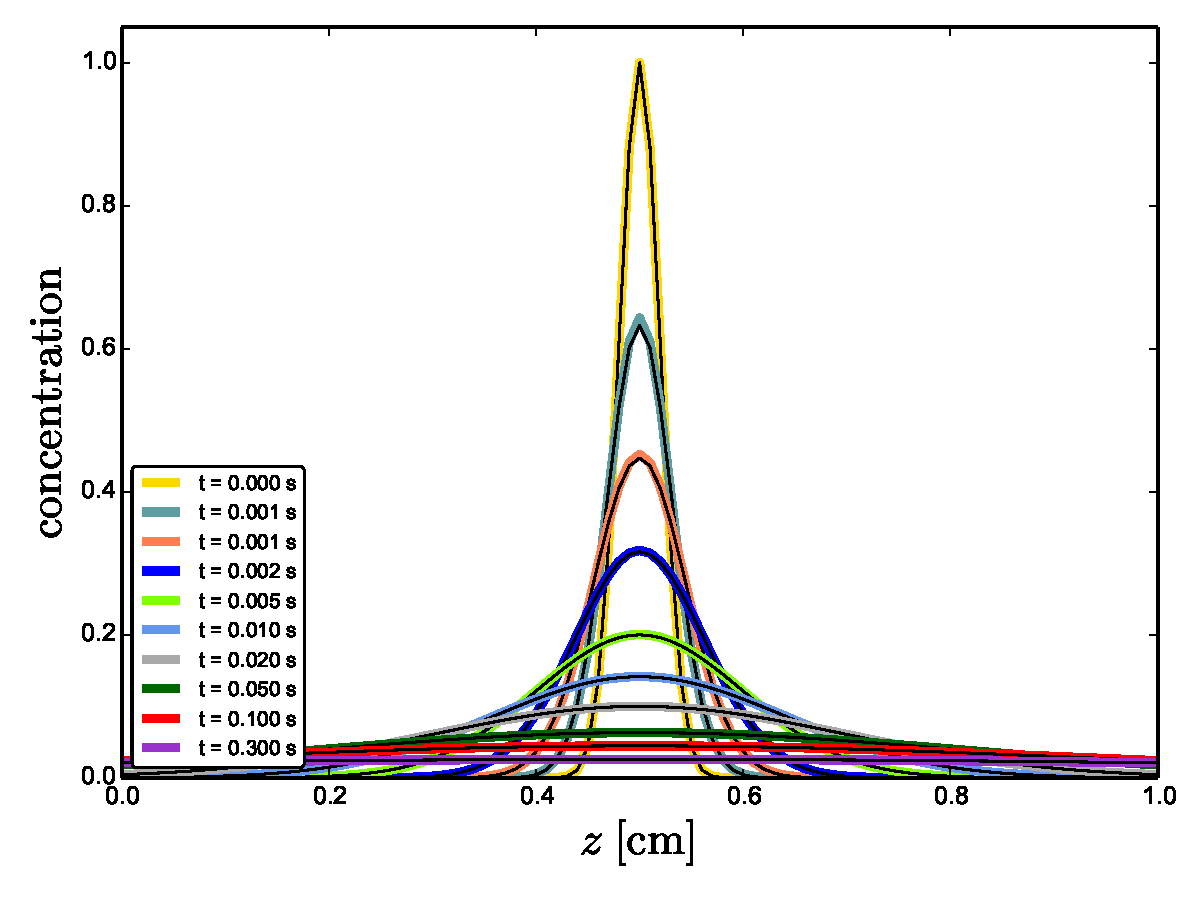
\includegraphics[width=16cm]{test4.pdf}\\[-5mm]
\caption{Diffusive evolution of an initial $\delta$-peak with
  analytic solution overplotted. The analytic solution is
  $\epsilon(z,t)=A(t)\exp\big(-(z\!-\!0.5)^2/w^2(t)\big)$ with
  $A(t)=\sqrt{t_0/t}$ and $w(t)=2\sqrt{D t}$.}
\label{fig4}
\end{figure}

\bibliographystyle{chicagon}
\bibliography{references}

\end{document}
